\documentclass[1p]{elsarticle_modified}
%\bibliographystyle{elsarticle-num}

%\usepackage[colorlinks]{hyperref}
%\usepackage{abbrmath_seonhwa} %\Abb, \Ascr, \Acal ,\Abf, \Afrak
\usepackage{amsfonts}
\usepackage{amssymb}
\usepackage{amsmath}
\usepackage{amsthm}
\usepackage{scalefnt}
\usepackage{amsbsy}
\usepackage{kotex}
\usepackage{caption}
\usepackage{subfig}
\usepackage{color}
\usepackage{graphicx}
\usepackage{xcolor} %% white, black, red, green, blue, cyan, magenta, yellow
\usepackage{float}
\usepackage{setspace}
\usepackage{hyperref}

\usepackage{tikz}
\usetikzlibrary{arrows}

\usepackage{multirow}
\usepackage{array} % fixed length table
\usepackage{hhline}

%%%%%%%%%%%%%%%%%%%%%
\makeatletter
\renewcommand*\env@matrix[1][\arraystretch]{%
	\edef\arraystretch{#1}%
	\hskip -\arraycolsep
	\let\@ifnextchar\new@ifnextchar
	\array{*\c@MaxMatrixCols c}}
\makeatother %https://tex.stackexchange.com/questions/14071/how-can-i-increase-the-line-spacing-in-a-matrix
%%%%%%%%%%%%%%%

\usepackage[normalem]{ulem}

\newcommand{\msout}[1]{\ifmmode\text{\sout{\ensuremath{#1}}}\else\sout{#1}\fi}
%SOURCE: \msout is \stkout macro in https://tex.stackexchange.com/questions/20609/strikeout-in-math-mode

\newcommand{\cancel}[1]{
	\ifmmode
	{\color{red}\msout{#1}}
	\else
	{\color{red}\sout{#1}}
	\fi
}

\newcommand{\add}[1]{
	{\color{blue}\uwave{#1}}
}

\newcommand{\replace}[2]{
	\ifmmode
	{\color{red}\msout{#1}}{\color{blue}\uwave{#2}}
	\else
	{\color{red}\sout{#1}}{\color{blue}\uwave{#2}}
	\fi
}

\newcommand{\Sol}{\mathcal{S}} %segment
\newcommand{\D}{D} %diagram
\newcommand{\A}{\mathcal{A}} %arc


%%%%%%%%%%%%%%%%%%%%%%%%%%%%%5 test

\def\sl{\operatorname{\textup{SL}}(2,\Cbb)}
\def\psl{\operatorname{\textup{PSL}}(2,\Cbb)}
\def\quan{\mkern 1mu \triangleright \mkern 1mu}

\theoremstyle{definition}
\newtheorem{thm}{Theorem}[section]
\newtheorem{prop}[thm]{Proposition}
\newtheorem{lem}[thm]{Lemma}
\newtheorem{ques}[thm]{Question}
\newtheorem{cor}[thm]{Corollary}
\newtheorem{defn}[thm]{Definition}
\newtheorem{exam}[thm]{Example}
\newtheorem{rmk}[thm]{Remark}
\newtheorem{alg}[thm]{Algorithm}

\newcommand{\I}{\sqrt{-1}}
\begin{document}

%\begin{frontmatter}
%
%\title{Boundary parabolic representations of knots up to 8 crossings}
%
%%% Group authors per affiliation:
%\author{Yunhi Cho} 
%\address{Department of Mathematics, University of Seoul, Seoul, Korea}
%\ead{yhcho@uos.ac.kr}
%
%
%\author{Seonhwa Kim} %\fnref{s_kim}}
%\address{Center for Geometry and Physics, Institute for Basic Science, Pohang, 37673, Korea}
%\ead{ryeona17@ibs.re.kr}
%
%\author{Hyuk Kim}
%\address{Department of Mathematical Sciences, Seoul National University, Seoul 08826, Korea}
%\ead{hyukkim@snu.ac.kr}
%
%\author{Seokbeom Yoon}
%\address{Department of Mathematical Sciences, Seoul National University, Seoul, 08826,  Korea}
%\ead{sbyoon15@snu.ac.kr}
%
%\begin{abstract}
%We find all boundary parabolic representation of knots up to 8 crossings.
%
%\end{abstract}
%\begin{keyword}
%    \MSC[2010] 57M25 
%\end{keyword}
%
%\end{frontmatter}

%\linenumbers
%\tableofcontents
%
\newcommand\colored[1]{\textcolor{white}{\rule[-0.35ex]{0.8em}{1.4ex}}\kern-0.8em\color{red} #1}%
%\newcommand\colored[1]{\textcolor{white}{ #1}\kern-2.17ex	\textcolor{white}{ #1}\kern-1.81ex	\textcolor{white}{ #1}\kern-2.15ex\color{red}#1	}

{\Large $\underline{12n_{0547}~(K12n_{0547})}$}

\setlength{\tabcolsep}{10pt}
\renewcommand{\arraystretch}{1.6}
\vspace{1cm}\begin{tabular}{m{100pt}>{\centering\arraybackslash}m{274pt}}
\multirow{5}{120pt}{
	\centering
	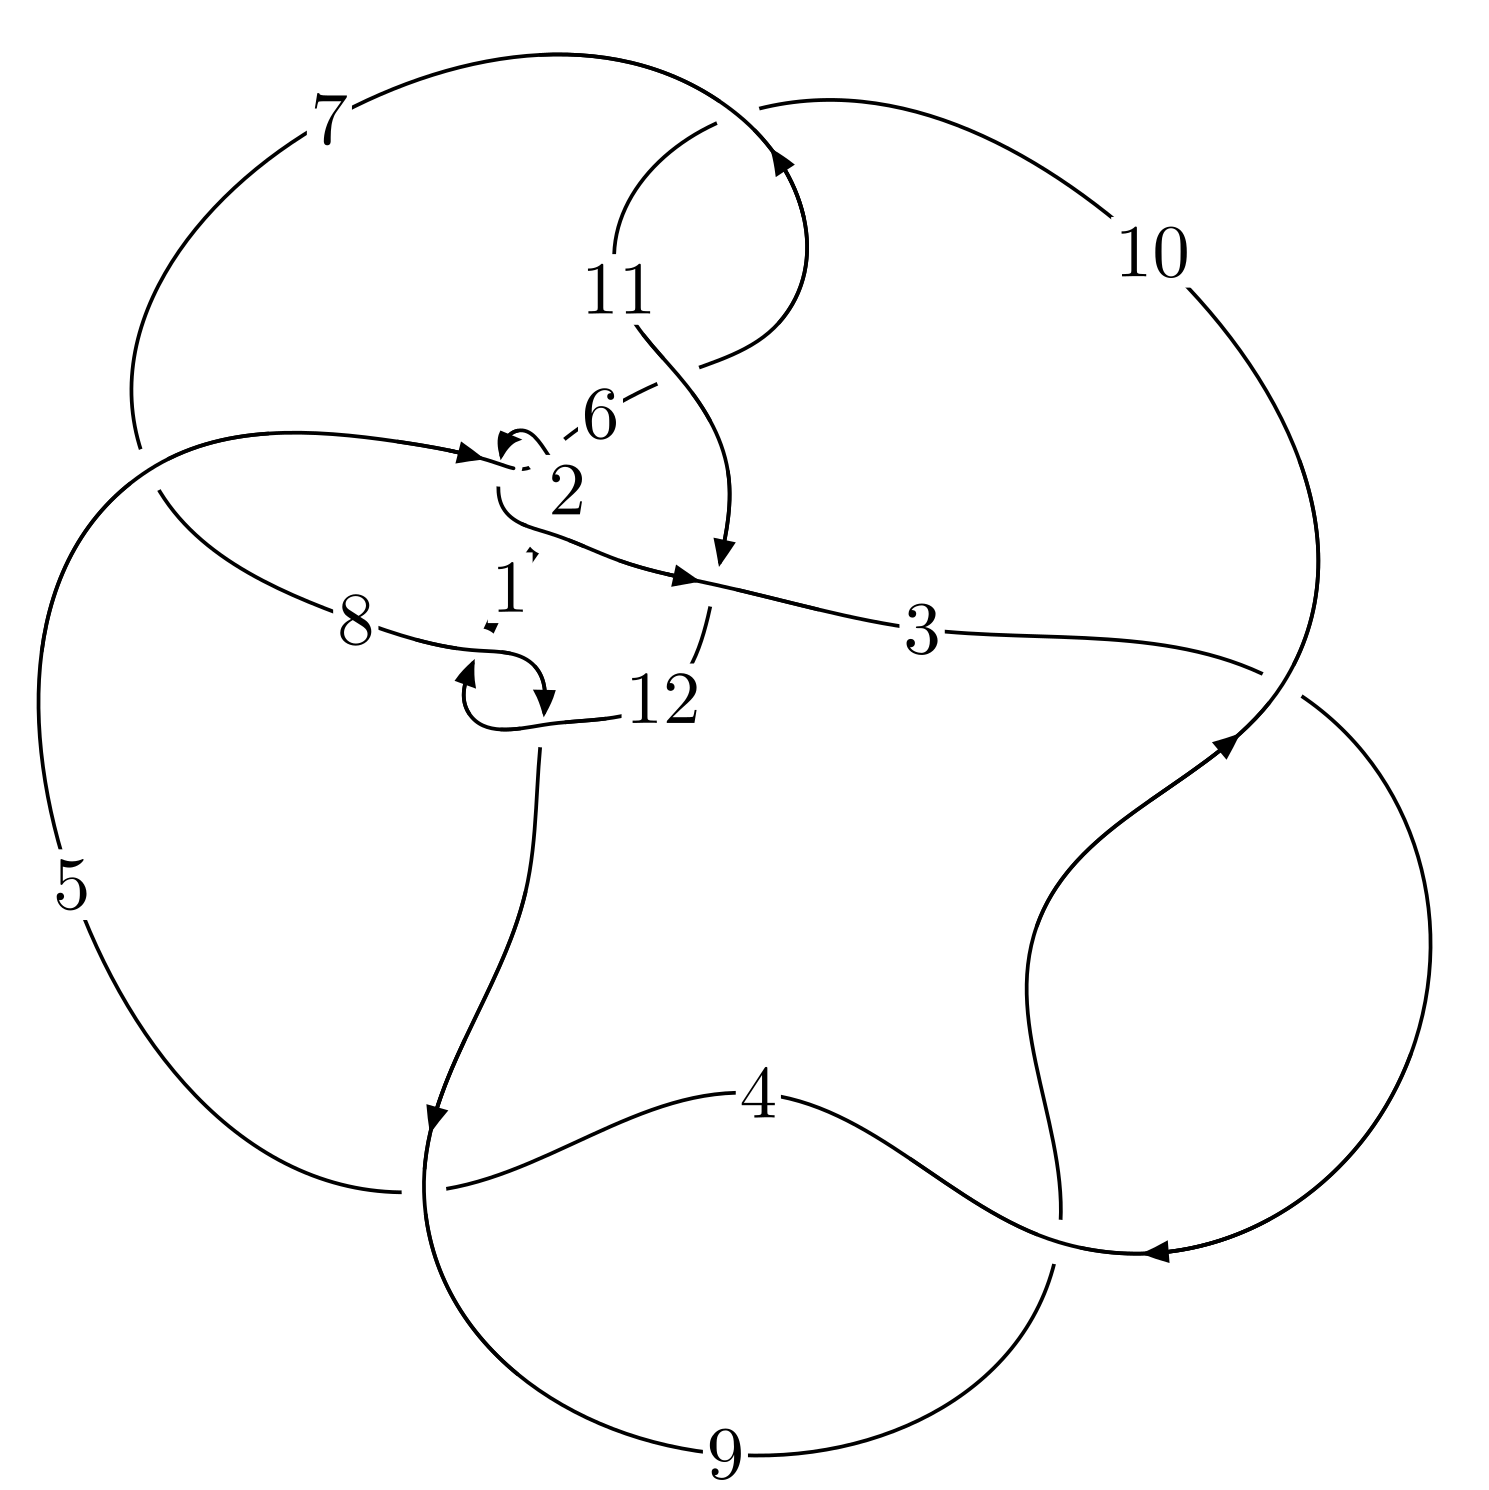
\includegraphics[width=112pt]{../../../GIT/diagram.site/Diagrams/png/2636_12n_0547.png}\\
\ \ \ A knot diagram\footnotemark}&
\allowdisplaybreaks
\textbf{Linearized knot diagam} \\
\cline{2-2}
 &
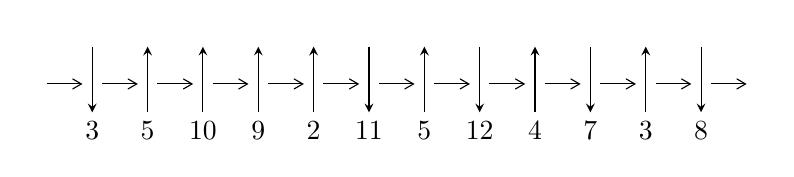
\begin{tikzpicture}[x=20pt, y=17pt]
	% nodes
	\node (C0) at (0, 0) {};
	\node (C1) at (1, 0) {};
	\node (C1U) at (1, +1) {};
	\node (C1D) at (1, -1) {3};

	\node (C2) at (2, 0) {};
	\node (C2U) at (2, +1) {};
	\node (C2D) at (2, -1) {5};

	\node (C3) at (3, 0) {};
	\node (C3U) at (3, +1) {};
	\node (C3D) at (3, -1) {10};

	\node (C4) at (4, 0) {};
	\node (C4U) at (4, +1) {};
	\node (C4D) at (4, -1) {9};

	\node (C5) at (5, 0) {};
	\node (C5U) at (5, +1) {};
	\node (C5D) at (5, -1) {2};

	\node (C6) at (6, 0) {};
	\node (C6U) at (6, +1) {};
	\node (C6D) at (6, -1) {11};

	\node (C7) at (7, 0) {};
	\node (C7U) at (7, +1) {};
	\node (C7D) at (7, -1) {5};

	\node (C8) at (8, 0) {};
	\node (C8U) at (8, +1) {};
	\node (C8D) at (8, -1) {12};

	\node (C9) at (9, 0) {};
	\node (C9U) at (9, +1) {};
	\node (C9D) at (9, -1) {4};

	\node (C10) at (10, 0) {};
	\node (C10U) at (10, +1) {};
	\node (C10D) at (10, -1) {7};

	\node (C11) at (11, 0) {};
	\node (C11U) at (11, +1) {};
	\node (C11D) at (11, -1) {3};

	\node (C12) at (12, 0) {};
	\node (C12U) at (12, +1) {};
	\node (C12D) at (12, -1) {8};
	\node (C13) at (13, 0) {};

	% arrows
	\draw[->,>={angle 60}]
	(C0) edge (C1) (C1) edge (C2) (C2) edge (C3) (C3) edge (C4) (C4) edge (C5) (C5) edge (C6) (C6) edge (C7) (C7) edge (C8) (C8) edge (C9) (C9) edge (C10) (C10) edge (C11) (C11) edge (C12) (C12) edge (C13) ;	\draw[->,>=stealth]
	(C1U) edge (C1D) (C2D) edge (C2U) (C3D) edge (C3U) (C4D) edge (C4U) (C5D) edge (C5U) (C6U) edge (C6D) (C7D) edge (C7U) (C8U) edge (C8D) (C9D) edge (C9U) (C10U) edge (C10D) (C11D) edge (C11U) (C12U) edge (C12D) ;
	\end{tikzpicture} \\
\hhline{~~} \\& 
\textbf{Solving Sequence} \\ \cline{2-2} 
 &
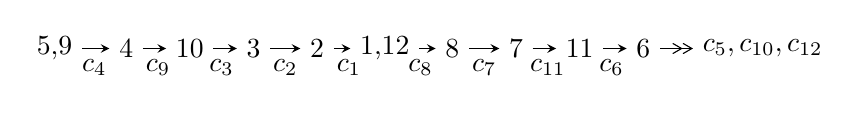
\begin{tikzpicture}[x=23pt, y=7pt]
	% node
	\node (A0) at (-1/8, 0) {5,9};
	\node (A1) at (1, 0) {4};
	\node (A2) at (2, 0) {10};
	\node (A3) at (3, 0) {3};
	\node (A4) at (4, 0) {2};
	\node (A5) at (81/16, 0) {1,12};
	\node (A6) at (49/8, 0) {8};
	\node (A7) at (57/8, 0) {7};
	\node (A8) at (65/8, 0) {11};
	\node (A9) at (73/8, 0) {6};
	\node (C1) at (1/2, -1) {$c_{4}$};
	\node (C2) at (3/2, -1) {$c_{9}$};
	\node (C3) at (5/2, -1) {$c_{3}$};
	\node (C4) at (7/2, -1) {$c_{2}$};
	\node (C5) at (9/2, -1) {$c_{1}$};
	\node (C6) at (45/8, -1) {$c_{8}$};
	\node (C7) at (53/8, -1) {$c_{7}$};
	\node (C8) at (61/8, -1) {$c_{11}$};
	\node (C9) at (69/8, -1) {$c_{6}$};
	\node (A10) at (11, 0) {$c_{5},c_{10},c_{12}$};

	% edge
	\draw[->,>=stealth]	
	(A0) edge (A1) (A1) edge (A2) (A2) edge (A3) (A3) edge (A4) (A4) edge (A5) (A5) edge (A6) (A6) edge (A7) (A7) edge (A8) (A8) edge (A9) ;
	\draw[->>,>={angle 60}]	
	(A9) edge (A10);
\end{tikzpicture} \\ 

\end{tabular} \\

\footnotetext{
The image of knot diagram is generated by the software ``\textbf{Draw programme}" developed by Andrew Bartholomew(\url{http://www.layer8.co.uk/maths/draw/index.htm\#Running-draw}), where we modified some parts for our purpose(\url{https://github.com/CATsTAILs/LinksPainter}).
}\phantom \\ \newline 
\centering \textbf{Ideals for irreducible components\footnotemark of $X_{\text{par}}$} 
 
\begin{align*}
I^u_{1}&=\langle 
- u^{18}+u^{17}+\cdots+b-1,\;u^{21}-3 u^{20}+\cdots+2 a-5,\;u^{22}-3 u^{21}+\cdots-7 u+2\rangle \\
I^u_{2}&=\langle 
u^9 a- u^{10}+\cdots+b-1,\\
\phantom{I^u_{2}}&\phantom{= \langle  }2 u^{10}+u^9+11 u^8+4 u^7+20 u^6+4 u^5- u^3 a+12 u^4-2 u^3+a^2-2 a u+3 u^2-3 u+5,\\
\phantom{I^u_{2}}&\phantom{= \langle  }u^{11}+u^{10}+6 u^9+5 u^8+12 u^7+8 u^6+8 u^5+3 u^4+u^3- u^2+2 u+1\rangle \\
I^u_{3}&=\langle 
- u^9+u^8-4 u^7+3 u^6-5 u^5- u^3-4 u^2+b+1,\;- u^8-4 u^6-5 u^4-2 u^2+a-1,\\
\phantom{I^u_{3}}&\phantom{= \langle  }u^{10}+5 u^8+8 u^6+3 u^4- u^2+1\rangle \\
\\
\end{align*}
\raggedright * 3 irreducible components of $\dim_{\mathbb{C}}=0$, with total 54 representations.\\
\footnotetext{All coefficients of polynomials are rational numbers. But the coefficients are sometimes approximated in decimal forms when there is not enough margin.}
\newpage
\renewcommand{\arraystretch}{1}
\centering \section*{I. $I^u_{1}= \langle - u^{18}+u^{17}+\cdots+b-1,\;u^{21}-3 u^{20}+\cdots+2 a-5,\;u^{22}-3 u^{21}+\cdots-7 u+2 \rangle$}
\flushleft \textbf{(i) Arc colorings}\\
\begin{tabular}{m{7pt} m{180pt} m{7pt} m{180pt} }
\flushright $a_{5}=$&$\begin{pmatrix}1\\0\end{pmatrix}$ \\
\flushright $a_{9}=$&$\begin{pmatrix}0\\u\end{pmatrix}$ \\
\flushright $a_{4}=$&$\begin{pmatrix}1\\u^2\end{pmatrix}$ \\
\flushright $a_{10}=$&$\begin{pmatrix}u\\u^3+u\end{pmatrix}$ \\
\flushright $a_{3}=$&$\begin{pmatrix}u^2+1\\u^4+2 u^2\end{pmatrix}$ \\
\flushright $a_{2}=$&$\begin{pmatrix}- u^4- u^2+1\\u^4+2 u^2\end{pmatrix}$ \\
\flushright $a_{1}=$&$\begin{pmatrix}u^{10}+5 u^8+8 u^6+3 u^4- u^2+1\\u^{12}+6 u^{10}+12 u^8+8 u^6+u^4+2 u^2\end{pmatrix}$ \\
\flushright $a_{12}=$&$\begin{pmatrix}-\frac{1}{2} u^{21}+\frac{3}{2} u^{20}+\cdots-4 u+\frac{5}{2}\\u^{18}- u^{17}+\cdots- u+1\end{pmatrix}$ \\
\flushright $a_{8}=$&$\begin{pmatrix}-\frac{1}{2} u^{21}+\frac{1}{2} u^{20}+\cdots- u-\frac{1}{2}\\- u^{21}+2 u^{20}+\cdots-3 u+1\end{pmatrix}$ \\
\flushright $a_{7}=$&$\begin{pmatrix}\frac{1}{2} u^{21}-\frac{3}{2} u^{20}+\cdots+2 u-\frac{3}{2}\\- u^{21}+2 u^{20}+\cdots-3 u+1\end{pmatrix}$ \\
\flushright $a_{11}=$&$\begin{pmatrix}\frac{1}{2} u^{21}-\frac{3}{2} u^{20}+\cdots+4 u-\frac{1}{2}\\- u^{18}+u^{17}+\cdots+2 u-1\end{pmatrix}$ \\
\flushright $a_{6}=$&$\begin{pmatrix}- u^8-3 u^6- u^4+2 u^2-1\\u^8+4 u^6+4 u^4\end{pmatrix}$\\&\end{tabular}
\flushleft \textbf{(ii) Obstruction class $= -1$}\\~\\
\flushleft \textbf{(iii) Cusp Shapes $= -4 u^{21}+10 u^{20}-54 u^{19}+108 u^{18}-298 u^{17}+482 u^{16}-868 u^{15}+1122 u^{14}-1404 u^{13}+1378 u^{12}-1148 u^{11}+700 u^{10}-226 u^9-136 u^8+252 u^7-198 u^6+68 u^5+44 u^4-74 u^3+56 u^2-34 u+14$}\\~\\
\newpage\renewcommand{\arraystretch}{1}
\flushleft \textbf{(iv) u-Polynomials at the component}\newline \\
\begin{tabular}{m{50pt}|m{274pt}}
Crossings & \hspace{64pt}u-Polynomials at each crossing \\
\hline $$\begin{aligned}c_{1}\end{aligned}$$&$\begin{aligned}
&u^{22}+21 u^{21}+\cdots+2639 u+576
\end{aligned}$\\
\hline $$\begin{aligned}c_{2},c_{5}\end{aligned}$$&$\begin{aligned}
&u^{22}+3 u^{21}+\cdots+55 u+24
\end{aligned}$\\
\hline $$\begin{aligned}c_{3},c_{4},c_{9}\end{aligned}$$&$\begin{aligned}
&u^{22}-3 u^{21}+\cdots-7 u+2
\end{aligned}$\\
\hline $$\begin{aligned}c_{6},c_{8},c_{10}\\c_{12}\end{aligned}$$&$\begin{aligned}
&u^{22}+2 u^{20}+\cdots+u+1
\end{aligned}$\\
\hline $$\begin{aligned}c_{7},c_{11}\end{aligned}$$&$\begin{aligned}
&u^{22}+4 u^{21}+\cdots-111 u+79
\end{aligned}$\\
\hline
\end{tabular}\\~\\
\newpage\renewcommand{\arraystretch}{1}
\flushleft \textbf{(v) Riley Polynomials at the component}\newline \\
\begin{tabular}{m{50pt}|m{274pt}}
Crossings & \hspace{64pt}Riley Polynomials at each crossing \\
\hline $$\begin{aligned}c_{1}\end{aligned}$$&$\begin{aligned}
&y^{22}-39 y^{21}+\cdots-969313 y+331776
\end{aligned}$\\
\hline $$\begin{aligned}c_{2},c_{5}\end{aligned}$$&$\begin{aligned}
&y^{22}+21 y^{21}+\cdots+2639 y+576
\end{aligned}$\\
\hline $$\begin{aligned}c_{3},c_{4},c_{9}\end{aligned}$$&$\begin{aligned}
&y^{22}+21 y^{21}+\cdots+7 y+4
\end{aligned}$\\
\hline $$\begin{aligned}c_{6},c_{8},c_{10}\\c_{12}\end{aligned}$$&$\begin{aligned}
&y^{22}+4 y^{21}+\cdots+11 y+1
\end{aligned}$\\
\hline $$\begin{aligned}c_{7},c_{11}\end{aligned}$$&$\begin{aligned}
&y^{22}+36 y^{21}+\cdots+103651 y+6241
\end{aligned}$\\
\hline
\end{tabular}\\~\\
\newpage\flushleft \textbf{(vi) Complex Volumes and Cusp Shapes}
$$\begin{array}{c|c|c}  
\text{Solutions to }I^u_{1}& \I (\text{vol} + \sqrt{-1}CS) & \text{Cusp shape}\\
 \hline 
\begin{aligned}
u &= \phantom{-}0.010224 + 1.078500 I \\
a &= \phantom{-}0.551130 + 0.398952 I \\
b &= -1.328730 - 0.305483 I\end{aligned}
 & -1.00862 + 1.46670 I & \phantom{-}0.87483 - 4.74244 I \\ \hline\begin{aligned}
u &= \phantom{-}0.010224 - 1.078500 I \\
a &= \phantom{-}0.551130 - 0.398952 I \\
b &= -1.328730 + 0.305483 I\end{aligned}
 & -1.00862 - 1.46670 I & \phantom{-}0.87483 + 4.74244 I \\ \hline\begin{aligned}
u &= \phantom{-}0.645447 + 0.555123 I \\
a &= -1.67610 - 0.24813 I \\
b &= -0.075830 - 0.925613 I\end{aligned}
 & -7.27791 - 5.01880 I & \phantom{-}0.42259 + 1.50295 I \\ \hline\begin{aligned}
u &= \phantom{-}0.645447 - 0.555123 I \\
a &= -1.67610 + 0.24813 I \\
b &= -0.075830 + 0.925613 I\end{aligned}
 & -7.27791 + 5.01880 I & \phantom{-}0.42259 - 1.50295 I \\ \hline\begin{aligned}
u &= \phantom{-}0.721588 + 0.445135 I \\
a &= \phantom{-}0.20635 - 1.70531 I \\
b &= \phantom{-}0.57553 - 1.93709 I\end{aligned}
 & -6.88868 + 9.58963 I & \phantom{-}1.41263 - 7.09128 I \\ \hline\begin{aligned}
u &= \phantom{-}0.721588 - 0.445135 I \\
a &= \phantom{-}0.20635 + 1.70531 I \\
b &= \phantom{-}0.57553 + 1.93709 I\end{aligned}
 & -6.88868 - 9.58963 I & \phantom{-}1.41263 + 7.09128 I \\ \hline\begin{aligned}
u &= -0.674386 + 0.184008 I \\
a &= -0.568999 - 1.273370 I \\
b &= -0.64562 - 1.59538 I\end{aligned}
 & \phantom{-}1.10963 - 4.53074 I & \phantom{-}4.38661 + 7.87378 I \\ \hline\begin{aligned}
u &= -0.674386 - 0.184008 I \\
a &= -0.568999 + 1.273370 I \\
b &= -0.64562 + 1.59538 I\end{aligned}
 & \phantom{-}1.10963 + 4.53074 I & \phantom{-}4.38661 - 7.87378 I \\ \hline\begin{aligned}
u &= -0.157344 + 0.613642 I \\
a &= \phantom{-}0.998496 + 0.716026 I \\
b &= -0.337730 - 0.250909 I\end{aligned}
 & -0.85003 + 1.30702 I & -1.78276 - 3.10332 I \\ \hline\begin{aligned}
u &= -0.157344 - 0.613642 I \\
a &= \phantom{-}0.998496 - 0.716026 I \\
b &= -0.337730 + 0.250909 I\end{aligned}
 & -0.85003 - 1.30702 I & -1.78276 + 3.10332 I\\
 \hline 
 \end{array}$$\newpage$$\begin{array}{c|c|c}  
\text{Solutions to }I^u_{1}& \I (\text{vol} + \sqrt{-1}CS) & \text{Cusp shape}\\
 \hline 
\begin{aligned}
u &= -0.261209 + 1.342740 I \\
a &= -0.524408 + 0.595373 I \\
b &= \phantom{-}2.12772 + 1.40190 I\end{aligned}
 & -3.69180 - 7.92861 I & -0.13268 + 8.49431 I \\ \hline\begin{aligned}
u &= -0.261209 - 1.342740 I \\
a &= -0.524408 - 0.595373 I \\
b &= \phantom{-}2.12772 - 1.40190 I\end{aligned}
 & -3.69180 + 7.92861 I & -0.13268 - 8.49431 I \\ \hline\begin{aligned}
u &= \phantom{-}0.587900 + 0.230513 I \\
a &= \phantom{-}0.564070 + 0.683652 I \\
b &= \phantom{-}0.173424 + 0.964850 I\end{aligned}
 & \phantom{-}1.14825 + 1.09478 I & \phantom{-}3.74609 - 1.33769 I \\ \hline\begin{aligned}
u &= \phantom{-}0.587900 - 0.230513 I \\
a &= \phantom{-}0.564070 - 0.683652 I \\
b &= \phantom{-}0.173424 - 0.964850 I\end{aligned}
 & \phantom{-}1.14825 - 1.09478 I & \phantom{-}3.74609 + 1.33769 I \\ \hline\begin{aligned}
u &= \phantom{-}0.22679 + 1.39926 I \\
a &= -0.435721 + 0.005462 I \\
b &= \phantom{-}0.901316 - 0.971219 I\end{aligned}
 & -4.08990 + 4.07620 I & -2.65002 - 1.63109 I \\ \hline\begin{aligned}
u &= \phantom{-}0.22679 - 1.39926 I \\
a &= -0.435721 - 0.005462 I \\
b &= \phantom{-}0.901316 + 0.971219 I\end{aligned}
 & -4.08990 - 4.07620 I & -2.65002 + 1.63109 I \\ \hline\begin{aligned}
u &= -0.06984 + 1.45133 I \\
a &= -0.328600 - 0.625258 I \\
b &= -0.008270 - 0.590017 I\end{aligned}
 & -7.21159 + 0.38553 I & -5.41030 - 1.50832 I \\ \hline\begin{aligned}
u &= -0.06984 - 1.45133 I \\
a &= -0.328600 + 0.625258 I \\
b &= -0.008270 + 0.590017 I\end{aligned}
 & -7.21159 - 0.38553 I & -5.41030 + 1.50832 I \\ \hline\begin{aligned}
u &= \phantom{-}0.26357 + 1.48721 I \\
a &= \phantom{-}0.667824 + 0.729458 I \\
b &= -1.59693 + 2.46692 I\end{aligned}
 & -13.1389 + 13.1870 I & -1.85056 - 6.97436 I \\ \hline\begin{aligned}
u &= \phantom{-}0.26357 - 1.48721 I \\
a &= \phantom{-}0.667824 - 0.729458 I \\
b &= -1.59693 - 2.46692 I\end{aligned}
 & -13.1389 - 13.1870 I & -1.85056 + 6.97436 I\\
 \hline 
 \end{array}$$\newpage$$\begin{array}{c|c|c}  
\text{Solutions to }I^u_{1}& \I (\text{vol} + \sqrt{-1}CS) & \text{Cusp shape}\\
 \hline 
\begin{aligned}
u &= \phantom{-}0.20725 + 1.51244 I \\
a &= \phantom{-}0.795966 - 0.560386 I \\
b &= \phantom{-}0.215117 - 0.125032 I\end{aligned}
 & -14.0282 - 1.9396 I & -3.01643 + 1.43017 I \\ \hline\begin{aligned}
u &= \phantom{-}0.20725 - 1.51244 I \\
a &= \phantom{-}0.795966 + 0.560386 I \\
b &= \phantom{-}0.215117 + 0.125032 I\end{aligned}
 & -14.0282 + 1.9396 I & -3.01643 - 1.43017 I\\
 \hline 
 \end{array}$$\newpage\newpage\renewcommand{\arraystretch}{1}
\centering \section*{II. $I^u_{2}= \langle u^9 a- u^{10}+\cdots+b-1,\;2 u^{10}+u^9+\cdots+a^2+5,\;u^{11}+u^{10}+\cdots+2 u+1 \rangle$}
\flushleft \textbf{(i) Arc colorings}\\
\begin{tabular}{m{7pt} m{180pt} m{7pt} m{180pt} }
\flushright $a_{5}=$&$\begin{pmatrix}1\\0\end{pmatrix}$ \\
\flushright $a_{9}=$&$\begin{pmatrix}0\\u\end{pmatrix}$ \\
\flushright $a_{4}=$&$\begin{pmatrix}1\\u^2\end{pmatrix}$ \\
\flushright $a_{10}=$&$\begin{pmatrix}u\\u^3+u\end{pmatrix}$ \\
\flushright $a_{3}=$&$\begin{pmatrix}u^2+1\\u^4+2 u^2\end{pmatrix}$ \\
\flushright $a_{2}=$&$\begin{pmatrix}- u^4- u^2+1\\u^4+2 u^2\end{pmatrix}$ \\
\flushright $a_{1}=$&$\begin{pmatrix}u^{10}+5 u^8+8 u^6+3 u^4- u^2+1\\u^{10}+u^9+5 u^8+4 u^7+8 u^6+5 u^5+3 u^4+2 u^3- u^2+u+1\end{pmatrix}$ \\
\flushright $a_{12}=$&$\begin{pmatrix}a\\- u^9 a+u^{10}+\cdots- a u+1\end{pmatrix}$ \\
\flushright $a_{8}=$&$\begin{pmatrix}u^{10}+u^9+\cdots- u+2\\- u^9 a- u^8 a+\cdots- a+1\end{pmatrix}$ \\
\flushright $a_{7}=$&$\begin{pmatrix}u^9 a+u^{10}+\cdots+a+1\\- u^9 a- u^8 a+\cdots- a+1\end{pmatrix}$ \\
\flushright $a_{11}=$&$\begin{pmatrix}u^9 a- u^{10}+\cdots+a-1\\- u^9 a+u^{10}+\cdots+u+1\end{pmatrix}$ \\
\flushright $a_{6}=$&$\begin{pmatrix}- u^8-3 u^6- u^4+2 u^2-1\\u^8+4 u^6+4 u^4\end{pmatrix}$\\&\end{tabular}
\flushleft \textbf{(ii) Obstruction class $= -1$}\\~\\
\flushleft \textbf{(iii) Cusp Shapes $= 4 u^{10}+4 u^9+24 u^8+16 u^7+44 u^6+16 u^5+20 u^4-4 u^3-4 u^2-4 u+10$}\\~\\
\newpage\renewcommand{\arraystretch}{1}
\flushleft \textbf{(iv) u-Polynomials at the component}\newline \\
\begin{tabular}{m{50pt}|m{274pt}}
Crossings & \hspace{64pt}u-Polynomials at each crossing \\
\hline $$\begin{aligned}c_{1}\end{aligned}$$&$\begin{aligned}
&(u^{11}+15 u^{10}+\cdots+6 u-1)^{2}
\end{aligned}$\\
\hline $$\begin{aligned}c_{2},c_{5}\end{aligned}$$&$\begin{aligned}
&(u^{11}+u^{10}+8 u^9+7 u^8+22 u^7+16 u^6+24 u^5+13 u^4+9 u^3+3 u^2-1)^2
\end{aligned}$\\
\hline $$\begin{aligned}c_{3},c_{4},c_{9}\end{aligned}$$&$\begin{aligned}
&(u^{11}+u^{10}+6 u^9+5 u^8+12 u^7+8 u^6+8 u^5+3 u^4+u^3- u^2+2 u+1)^2
\end{aligned}$\\
\hline $$\begin{aligned}c_{6},c_{8},c_{10}\\c_{12}\end{aligned}$$&$\begin{aligned}
&u^{22}+u^{21}+\cdots+20 u^3+1
\end{aligned}$\\
\hline $$\begin{aligned}c_{7},c_{11}\end{aligned}$$&$\begin{aligned}
&u^{22}+u^{21}+\cdots+3324 u+5777
\end{aligned}$\\
\hline
\end{tabular}\\~\\
\newpage\renewcommand{\arraystretch}{1}
\flushleft \textbf{(v) Riley Polynomials at the component}\newline \\
\begin{tabular}{m{50pt}|m{274pt}}
Crossings & \hspace{64pt}Riley Polynomials at each crossing \\
\hline $$\begin{aligned}c_{1}\end{aligned}$$&$\begin{aligned}
&(y^{11}-37 y^{10}+\cdots+70 y-1)^{2}
\end{aligned}$\\
\hline $$\begin{aligned}c_{2},c_{5}\end{aligned}$$&$\begin{aligned}
&(y^{11}+15 y^{10}+\cdots+6 y-1)^{2}
\end{aligned}$\\
\hline $$\begin{aligned}c_{3},c_{4},c_{9}\end{aligned}$$&$\begin{aligned}
&(y^{11}+11 y^{10}+\cdots+6 y-1)^{2}
\end{aligned}$\\
\hline $$\begin{aligned}c_{6},c_{8},c_{10}\\c_{12}\end{aligned}$$&$\begin{aligned}
&y^{22}+7 y^{21}+\cdots+84 y^2+1
\end{aligned}$\\
\hline $$\begin{aligned}c_{7},c_{11}\end{aligned}$$&$\begin{aligned}
&y^{22}+11 y^{21}+\cdots+10487680 y+33373729
\end{aligned}$\\
\hline
\end{tabular}\\~\\
\newpage\flushleft \textbf{(vi) Complex Volumes and Cusp Shapes}
$$\begin{array}{c|c|c}  
\text{Solutions to }I^u_{2}& \I (\text{vol} + \sqrt{-1}CS) & \text{Cusp shape}\\
 \hline 
\begin{aligned}
u &= -0.691368 + 0.499908 I \\
a &= -1.59688 + 0.02132 I \\
b &= -0.638758 + 0.617238 I\end{aligned}
 & -7.95553 - 2.30219 I & -0.32022 + 2.86330 I \\ \hline\begin{aligned}
u &= -0.691368 + 0.499908 I \\
a &= \phantom{-}0.40201 + 1.57042 I \\
b &= \phantom{-}0.73852 + 1.27823 I\end{aligned}
 & -7.95553 - 2.30219 I & -0.32022 + 2.86330 I \\ \hline\begin{aligned}
u &= -0.691368 - 0.499908 I \\
a &= -1.59688 - 0.02132 I \\
b &= -0.638758 - 0.617238 I\end{aligned}
 & -7.95553 + 2.30219 I & -0.32022 - 2.86330 I \\ \hline\begin{aligned}
u &= -0.691368 - 0.499908 I \\
a &= \phantom{-}0.40201 - 1.57042 I \\
b &= \phantom{-}0.73852 - 1.27823 I\end{aligned}
 & -7.95553 + 2.30219 I & -0.32022 - 2.86330 I \\ \hline\begin{aligned}
u &= -0.081634 + 1.321480 I \\
a &= \phantom{-}0.925705 + 0.046443 I \\
b &= -2.41105 - 0.00160 I\end{aligned}
 & -0.18031 - 1.62554 I & \phantom{-}1.42199 + 3.91435 I \\ \hline\begin{aligned}
u &= -0.081634 + 1.321480 I \\
a &= -0.661845 + 0.315235 I \\
b &= \phantom{-}0.12364 + 2.65077 I\end{aligned}
 & -0.18031 - 1.62554 I & \phantom{-}1.42199 + 3.91435 I \\ \hline\begin{aligned}
u &= -0.081634 - 1.321480 I \\
a &= \phantom{-}0.925705 - 0.046443 I \\
b &= -2.41105 + 0.00160 I\end{aligned}
 & -0.18031 + 1.62554 I & \phantom{-}1.42199 - 3.91435 I \\ \hline\begin{aligned}
u &= -0.081634 - 1.321480 I \\
a &= -0.661845 - 0.315235 I \\
b &= \phantom{-}0.12364 - 2.65077 I\end{aligned}
 & -0.18031 + 1.62554 I & \phantom{-}1.42199 - 3.91435 I \\ \hline\begin{aligned}
u &= \phantom{-}0.525209 + 0.369457 I \\
a &= \phantom{-}0.073929 - 0.488809 I \\
b &= -0.422255 + 0.248502 I\end{aligned}
 & \phantom{-}1.26759 + 1.65848 I & \phantom{-}0.54419 - 4.72916 I \\ \hline\begin{aligned}
u &= \phantom{-}0.525209 + 0.369457 I \\
a &= \phantom{-}0.90630 + 1.48303 I \\
b &= -0.128441 + 1.396340 I\end{aligned}
 & \phantom{-}1.26759 + 1.65848 I & \phantom{-}0.54419 - 4.72916 I\\
 \hline 
 \end{array}$$\newpage$$\begin{array}{c|c|c}  
\text{Solutions to }I^u_{2}& \I (\text{vol} + \sqrt{-1}CS) & \text{Cusp shape}\\
 \hline 
\begin{aligned}
u &= \phantom{-}0.525209 - 0.369457 I \\
a &= \phantom{-}0.073929 + 0.488809 I \\
b &= -0.422255 - 0.248502 I\end{aligned}
 & \phantom{-}1.26759 - 1.65848 I & \phantom{-}0.54419 + 4.72916 I \\ \hline\begin{aligned}
u &= \phantom{-}0.525209 - 0.369457 I \\
a &= \phantom{-}0.90630 - 1.48303 I \\
b &= -0.128441 - 1.396340 I\end{aligned}
 & \phantom{-}1.26759 - 1.65848 I & \phantom{-}0.54419 + 4.72916 I \\ \hline\begin{aligned}
u &= \phantom{-}0.18554 + 1.42716 I \\
a &= -0.752259 - 0.261413 I \\
b &= \phantom{-}1.03684 - 1.52064 I\end{aligned}
 & -4.47712 + 4.26374 I & -2.95029 - 4.02329 I \\ \hline\begin{aligned}
u &= \phantom{-}0.18554 + 1.42716 I \\
a &= -0.003996 + 0.356321 I \\
b &= \phantom{-}0.624973 + 0.515135 I\end{aligned}
 & -4.47712 + 4.26374 I & -2.95029 - 4.02329 I \\ \hline\begin{aligned}
u &= \phantom{-}0.18554 - 1.42716 I \\
a &= -0.752259 + 0.261413 I \\
b &= \phantom{-}1.03684 + 1.52064 I\end{aligned}
 & -4.47712 - 4.26374 I & -2.95029 + 4.02329 I \\ \hline\begin{aligned}
u &= \phantom{-}0.18554 - 1.42716 I \\
a &= -0.003996 - 0.356321 I \\
b &= \phantom{-}0.624973 - 0.515135 I\end{aligned}
 & -4.47712 - 4.26374 I & -2.95029 + 4.02329 I \\ \hline\begin{aligned}
u &= -0.23988 + 1.50376 I \\
a &= \phantom{-}0.504184 - 0.804775 I \\
b &= -1.21612 - 1.84606 I\end{aligned}
 & -14.4695 - 5.6984 I & -3.54476 + 2.83577 I \\ \hline\begin{aligned}
u &= -0.23988 + 1.50376 I \\
a &= \phantom{-}0.629578 + 0.671456 I \\
b &= \phantom{-}0.849788 + 0.004381 I\end{aligned}
 & -14.4695 - 5.6984 I & -3.54476 + 2.83577 I \\ \hline\begin{aligned}
u &= -0.23988 - 1.50376 I \\
a &= \phantom{-}0.504184 + 0.804775 I \\
b &= -1.21612 + 1.84606 I\end{aligned}
 & -14.4695 + 5.6984 I & -3.54476 - 2.83577 I \\ \hline\begin{aligned}
u &= -0.23988 - 1.50376 I \\
a &= \phantom{-}0.629578 - 0.671456 I \\
b &= \phantom{-}0.849788 - 0.004381 I\end{aligned}
 & -14.4695 + 5.6984 I & -3.54476 - 2.83577 I\\
 \hline 
 \end{array}$$\newpage$$\begin{array}{c|c|c}  
\text{Solutions to }I^u_{2}& \I (\text{vol} + \sqrt{-1}CS) & \text{Cusp shape}\\
 \hline 
\begin{aligned}
u &= -0.395736\phantom{ +0.000000I} \\
a &= -0.42672 + 2.63281 I \\
b &= \phantom{-}0.94286 + 1.41200 I\end{aligned}
 & \phantom{-}3.92670\phantom{ +0.000000I} & \phantom{-}11.6980\phantom{ +0.000000I} \\ \hline\begin{aligned}
u &= -0.395736\phantom{ +0.000000I} \\
a &= -0.42672 - 2.63281 I \\
b &= \phantom{-}0.94286 - 1.41200 I\end{aligned}
 & \phantom{-}3.92670\phantom{ +0.000000I} & \phantom{-}11.6980\phantom{ +0.000000I}\\
 \hline 
 \end{array}$$\newpage\newpage\renewcommand{\arraystretch}{1}
\centering \section*{III. $I^u_{3}= \langle - u^9+u^8+\cdots+b+1,\;- u^8-4 u^6-5 u^4-2 u^2+a-1,\;u^{10}+5 u^8+8 u^6+3 u^4- u^2+1 \rangle$}
\flushleft \textbf{(i) Arc colorings}\\
\begin{tabular}{m{7pt} m{180pt} m{7pt} m{180pt} }
\flushright $a_{5}=$&$\begin{pmatrix}1\\0\end{pmatrix}$ \\
\flushright $a_{9}=$&$\begin{pmatrix}0\\u\end{pmatrix}$ \\
\flushright $a_{4}=$&$\begin{pmatrix}1\\u^2\end{pmatrix}$ \\
\flushright $a_{10}=$&$\begin{pmatrix}u\\u^3+u\end{pmatrix}$ \\
\flushright $a_{3}=$&$\begin{pmatrix}u^2+1\\u^4+2 u^2\end{pmatrix}$ \\
\flushright $a_{2}=$&$\begin{pmatrix}- u^4- u^2+1\\u^4+2 u^2\end{pmatrix}$ \\
\flushright $a_{1}=$&$\begin{pmatrix}0\\- u^8-3 u^6- u^4+2 u^2-1\end{pmatrix}$ \\
\flushright $a_{12}=$&$\begin{pmatrix}u^8+4 u^6+5 u^4+2 u^2+1\\u^9- u^8+4 u^7-3 u^6+5 u^5+u^3+4 u^2-1\end{pmatrix}$ \\
\flushright $a_{8}=$&$\begin{pmatrix}u^9+5 u^7+8 u^5+3 u^3- u\\- u^8+u^7-4 u^6+3 u^5-4 u^4+2 u^3- u-1\end{pmatrix}$ \\
\flushright $a_{7}=$&$\begin{pmatrix}u^9+u^8+4 u^7+4 u^6+5 u^5+4 u^4+u^3+1\\- u^8+u^7-4 u^6+3 u^5-4 u^4+2 u^3- u-1\end{pmatrix}$ \\
\flushright $a_{11}=$&$\begin{pmatrix}- u^9+u^8-4 u^7+4 u^6-5 u^5+4 u^4- u^3+u+1\\u^9+4 u^7+5 u^5+u^4+2 u^3+2 u^2+u\end{pmatrix}$ \\
\flushright $a_{6}=$&$\begin{pmatrix}u^8+3 u^6+u^4-2 u^2+1\\- u^8-4 u^6-4 u^4\end{pmatrix}$\\&\end{tabular}
\flushleft \textbf{(ii) Obstruction class $= 1$}\\~\\
\flushleft \textbf{(iii) Cusp Shapes $= -4 u^6-12 u^4-8 u^2+8$}\\~\\
\newpage\renewcommand{\arraystretch}{1}
\flushleft \textbf{(iv) u-Polynomials at the component}\newline \\
\begin{tabular}{m{50pt}|m{274pt}}
Crossings & \hspace{64pt}u-Polynomials at each crossing \\
\hline $$\begin{aligned}c_{1}\end{aligned}$$&$\begin{aligned}
&(u^5-3 u^4+4 u^3- u^2- u+1)^2
\end{aligned}$\\
\hline $$\begin{aligned}c_{2}\end{aligned}$$&$\begin{aligned}
&(u^5- u^4+2 u^3- u^2+u-1)^2
\end{aligned}$\\
\hline $$\begin{aligned}c_{3},c_{4},c_{9}\end{aligned}$$&$\begin{aligned}
&u^{10}+5 u^8+8 u^6+3 u^4- u^2+1
\end{aligned}$\\
\hline $$\begin{aligned}c_{5}\end{aligned}$$&$\begin{aligned}
&(u^5+u^4+2 u^3+u^2+u+1)^2
\end{aligned}$\\
\hline $$\begin{aligned}c_{6},c_{8},c_{10}\\c_{12}\end{aligned}$$&$\begin{aligned}
&(u^2+1)^5
\end{aligned}$\\
\hline $$\begin{aligned}c_{7}\end{aligned}$$&$\begin{aligned}
&u^{10}-4 u^9+\cdots-74 u+29
\end{aligned}$\\
\hline $$\begin{aligned}c_{11}\end{aligned}$$&$\begin{aligned}
&u^{10}+4 u^9+\cdots+74 u+29
\end{aligned}$\\
\hline
\end{tabular}\\~\\
\newpage\renewcommand{\arraystretch}{1}
\flushleft \textbf{(v) Riley Polynomials at the component}\newline \\
\begin{tabular}{m{50pt}|m{274pt}}
Crossings & \hspace{64pt}Riley Polynomials at each crossing \\
\hline $$\begin{aligned}c_{1}\end{aligned}$$&$\begin{aligned}
&(y^5- y^4+8 y^3-3 y^2+3 y-1)^2
\end{aligned}$\\
\hline $$\begin{aligned}c_{2},c_{5}\end{aligned}$$&$\begin{aligned}
&(y^5+3 y^4+4 y^3+y^2- y-1)^2
\end{aligned}$\\
\hline $$\begin{aligned}c_{3},c_{4},c_{9}\end{aligned}$$&$\begin{aligned}
&(y^5+5 y^4+8 y^3+3 y^2- y+1)^2
\end{aligned}$\\
\hline $$\begin{aligned}c_{6},c_{8},c_{10}\\c_{12}\end{aligned}$$&$\begin{aligned}
&(y+1)^{10}
\end{aligned}$\\
\hline $$\begin{aligned}c_{7},c_{11}\end{aligned}$$&$\begin{aligned}
&y^{10}-6 y^9+\cdots-546 y+841
\end{aligned}$\\
\hline
\end{tabular}\\~\\
\newpage\flushleft \textbf{(vi) Complex Volumes and Cusp Shapes}
$$\begin{array}{c|c|c}  
\text{Solutions to }I^u_{3}& \I (\text{vol} + \sqrt{-1}CS) & \text{Cusp shape}\\
 \hline 
\begin{aligned}
u &= \phantom{-0.000000 -}1.217740 I \\
a &= \phantom{-}0.821196\phantom{ +0.000000I} \\
b &= -1.98456 + 1.58802 I\end{aligned}
 & \phantom{-}0.888787\phantom{ +0.000000I} & \phantom{-}6.51890\phantom{ +0.000000I} \\ \hline\begin{aligned}
u &= \phantom{-0.000000 } -1.217740 I \\
a &= \phantom{-}0.821196\phantom{ +0.000000I} \\
b &= -1.98456 - 1.58802 I\end{aligned}
 & \phantom{-}0.888787\phantom{ +0.000000I} & \phantom{-}6.51890\phantom{ +0.000000I} \\ \hline\begin{aligned}
u &= \phantom{-}0.549911 + 0.309916 I \\
a &= \phantom{-}0.77780 + 1.38013 I \\
b &= -0.52856 + 1.81098 I\end{aligned}
 & \phantom{-}2.96077 + 1.53058 I & \phantom{-}7.48489 - 4.43065 I \\ \hline\begin{aligned}
u &= \phantom{-}0.549911 - 0.309916 I \\
a &= \phantom{-}0.77780 - 1.38013 I \\
b &= -0.52856 - 1.81098 I\end{aligned}
 & \phantom{-}2.96077 - 1.53058 I & \phantom{-}7.48489 + 4.43065 I \\ \hline\begin{aligned}
u &= -0.549911 + 0.309916 I \\
a &= \phantom{-}0.77780 - 1.38013 I \\
b &= \phantom{-}0.586946 - 0.933592 I\end{aligned}
 & \phantom{-}2.96077 - 1.53058 I & \phantom{-}7.48489 + 4.43065 I \\ \hline\begin{aligned}
u &= -0.549911 - 0.309916 I \\
a &= \phantom{-}0.77780 + 1.38013 I \\
b &= \phantom{-}0.586946 + 0.933592 I\end{aligned}
 & \phantom{-}2.96077 + 1.53058 I & \phantom{-}7.48489 - 4.43065 I \\ \hline\begin{aligned}
u &= -0.21917 + 1.41878 I \\
a &= -0.688402 + 0.106340 I \\
b &= -0.13073 + 1.65202 I\end{aligned}
 & -2.58269 - 4.40083 I & \phantom{-}3.25569 + 3.49859 I \\ \hline\begin{aligned}
u &= -0.21917 - 1.41878 I \\
a &= -0.688402 - 0.106340 I \\
b &= -0.13073 - 1.65202 I\end{aligned}
 & -2.58269 + 4.40083 I & \phantom{-}3.25569 - 3.49859 I \\ \hline\begin{aligned}
u &= \phantom{-}0.21917 + 1.41878 I \\
a &= -0.688402 - 0.106340 I \\
b &= \phantom{-}2.05690 - 1.18661 I\end{aligned}
 & -2.58269 + 4.40083 I & \phantom{-}3.25569 - 3.49859 I \\ \hline\begin{aligned}
u &= \phantom{-}0.21917 - 1.41878 I \\
a &= -0.688402 + 0.106340 I \\
b &= \phantom{-}2.05690 + 1.18661 I\end{aligned}
 & -2.58269 - 4.40083 I & \phantom{-}3.25569 + 3.49859 I\\
 \hline 
 \end{array}$$\newpage
\newpage\renewcommand{\arraystretch}{1}
\centering \section*{ IV. u-Polynomials}
\begin{tabular}{m{50pt}|m{274pt}}
Crossings & \hspace{64pt}u-Polynomials at each crossing \\
\hline $$\begin{aligned}c_{1}\end{aligned}$$&$\begin{aligned}
&((u^5-3 u^4+4 u^3- u^2- u+1)^2)(u^{11}+15 u^{10}+\cdots+6 u-1)^{2}\\
&\cdot(u^{22}+21 u^{21}+\cdots+2639 u+576)
\end{aligned}$\\
\hline $$\begin{aligned}c_{2}\end{aligned}$$&$\begin{aligned}
&(u^5- u^4+2 u^3- u^2+u-1)^2\\
&\cdot(u^{11}+u^{10}+8 u^9+7 u^8+22 u^7+16 u^6+24 u^5+13 u^4+9 u^3+3 u^2-1)^2\\
&\cdot(u^{22}+3 u^{21}+\cdots+55 u+24)
\end{aligned}$\\
\hline $$\begin{aligned}c_{3},c_{4},c_{9}\end{aligned}$$&$\begin{aligned}
&(u^{10}+5 u^8+8 u^6+3 u^4- u^2+1)\\
&\cdot(u^{11}+u^{10}+6 u^9+5 u^8+12 u^7+8 u^6+8 u^5+3 u^4+u^3- u^2+2 u+1)^2\\
&\cdot(u^{22}-3 u^{21}+\cdots-7 u+2)
\end{aligned}$\\
\hline $$\begin{aligned}c_{5}\end{aligned}$$&$\begin{aligned}
&(u^5+u^4+2 u^3+u^2+u+1)^2\\
&\cdot(u^{11}+u^{10}+8 u^9+7 u^8+22 u^7+16 u^6+24 u^5+13 u^4+9 u^3+3 u^2-1)^2\\
&\cdot(u^{22}+3 u^{21}+\cdots+55 u+24)
\end{aligned}$\\
\hline $$\begin{aligned}c_{6},c_{8},c_{10}\\c_{12}\end{aligned}$$&$\begin{aligned}
&((u^2+1)^5)(u^{22}+2 u^{20}+\cdots+u+1)(u^{22}+u^{21}+\cdots+20 u^3+1)
\end{aligned}$\\
\hline $$\begin{aligned}c_{7}\end{aligned}$$&$\begin{aligned}
&(u^{10}-4 u^9+\cdots-74 u+29)(u^{22}+u^{21}+\cdots+3324 u+5777)\\
&\cdot(u^{22}+4 u^{21}+\cdots-111 u+79)
\end{aligned}$\\
\hline $$\begin{aligned}c_{11}\end{aligned}$$&$\begin{aligned}
&(u^{10}+4 u^9+\cdots+74 u+29)(u^{22}+u^{21}+\cdots+3324 u+5777)\\
&\cdot(u^{22}+4 u^{21}+\cdots-111 u+79)
\end{aligned}$\\
\hline
\end{tabular}\newpage\renewcommand{\arraystretch}{1}
\centering \section*{ V. Riley Polynomials}
\begin{tabular}{m{50pt}|m{274pt}}
Crossings & \hspace{64pt}Riley Polynomials at each crossing \\
\hline $$\begin{aligned}c_{1}\end{aligned}$$&$\begin{aligned}
&((y^5- y^4+8 y^3-3 y^2+3 y-1)^2)(y^{11}-37 y^{10}+\cdots+70 y-1)^{2}\\
&\cdot(y^{22}-39 y^{21}+\cdots-969313 y+331776)
\end{aligned}$\\
\hline $$\begin{aligned}c_{2},c_{5}\end{aligned}$$&$\begin{aligned}
&((y^5+3 y^4+4 y^3+y^2- y-1)^2)(y^{11}+15 y^{10}+\cdots+6 y-1)^{2}\\
&\cdot(y^{22}+21 y^{21}+\cdots+2639 y+576)
\end{aligned}$\\
\hline $$\begin{aligned}c_{3},c_{4},c_{9}\end{aligned}$$&$\begin{aligned}
&((y^5+5 y^4+8 y^3+3 y^2- y+1)^2)(y^{11}+11 y^{10}+\cdots+6 y-1)^{2}\\
&\cdot(y^{22}+21 y^{21}+\cdots+7 y+4)
\end{aligned}$\\
\hline $$\begin{aligned}c_{6},c_{8},c_{10}\\c_{12}\end{aligned}$$&$\begin{aligned}
&((y+1)^{10})(y^{22}+4 y^{21}+\cdots+11 y+1)(y^{22}+7 y^{21}+\cdots+84 y^2+1)
\end{aligned}$\\
\hline $$\begin{aligned}c_{7},c_{11}\end{aligned}$$&$\begin{aligned}
&(y^{10}-6 y^9+\cdots-546 y+841)\\
&\cdot(y^{22}+11 y^{21}+\cdots+10487680 y+33373729)\\
&\cdot(y^{22}+36 y^{21}+\cdots+103651 y+6241)
\end{aligned}$\\
\hline
\end{tabular}
\vskip 2pc
\end{document}